\documentclass{article}
\usepackage[utf8]{inputenc}
\usepackage{geometry}
\usepackage{tikz}

\usepackage{graphicx}
\graphicspath{{images/}}

\usepackage{float}
\usepackage{caption}
\usepackage{subcaption}
\captionsetup{compatibility=false}

\usepackage{hyperref}
\hypersetup{
  colorlinks,
  citecolor=black,
  filecolor=black,
  linkcolor=black,
  urlcolor=blue
}

\title{Polytope}
\author{URL, Mathtician, }
\date{February 2021}

\begin{document}

\maketitle

\section{Introduction}
Welcome to the \href{https://discord.gg/invite/zMRu7T4}{Polytope Discord}!

\section{What is a polytope?}
Roughly speaking, a \textbf{polytope} is an $n$-dimensional shape.
As with many terms used on the Polytope Discord,
the word ``polytope'' can have a few definitions which are not completely equivalent.
All of the commonly-used ones, however, agree:
\begin{enumerate}
  \item
A polytope in $n$ dimensions (known hereafter as an $n$-polytope)
is made of \textbf{facets} which are $(n-1)$-polytopes.
\begin{itemize}
\item \textbf{Points} ($0$-polytopes) are the facets of \textbf{line segments} ($1$-polytopes),
\item which are the facets of \textbf{polygons} ($2$-polytopes),
\item which are the facets of \textbf{polyhedra} ($3$-polytopes),
\item which are the facets of \textbf{polychora} ($4$-polytopes), etc.
\end{itemize}
For the next criterion, consider the following figures ABC and DEF.
\end{enumerate}

\begin{center}
  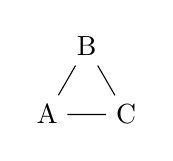
\begin{tikzpicture}
    \node (a) at (0,0) {A};
    \node (b) at (0.5,0.866) {B};
    \node (c) at (1,0) {C};
    \draw (a) -- (b) -- (c) -- (a);
  \end{tikzpicture}
  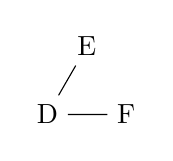
\begin{tikzpicture}
    \node (d) at (0,0) {D};
    \node (e) at (0.5,0.866) {E};
    \node (f) at (1,0) {F};
    \draw (e) -- (d) -- (f);
  \end{tikzpicture}
\end{center}

ABC is a triangle, a polygon with three line segments,
or \textbf{edges}, as they are known when mentioned as part of a larger polytope.
It also contains three points, or \textbf{vertices}, or even \textbf{verts} for short.
(In the polytope world, abbreviations are everywhere!)
DEF, on the other hand, is not a triangle; it is missing an edge,
leaving ``open ends'' at E and F which are each connected to only one edge.
To exclude DEF and figures like it,
we require that within a polygon, every vertex be connected to exactly two edges.
This condition also excludes ``branches'' where more than two edges meet at a vertex.

Let's generalize this rule to $n$-dimensional polytopes.
Two 3D figures are shown below.

\begin{center}
  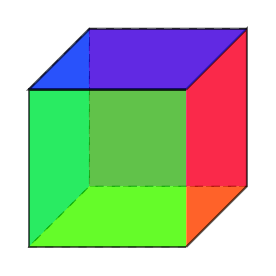
\begin{tikzpicture}
    \coordinate (A0) at (1,1,1);
    \coordinate (A1) at (1,1,-1);
    \coordinate (A2) at (1,-1,1);
    \coordinate (A3) at (1,-1,-1);
    \coordinate (A4) at (-1,1,1);
    \coordinate (A5) at (-1,1,-1);
    \coordinate (A6) at (-1,-1,1);
    \coordinate (A7) at (-1,-1,-1);
    \draw[dashed,fill=cyan,opacity=0.6] (A4) -- (A5) -- (A7) -- (A6);
    \draw[dashed,fill=magenta,opacity=0.6] (A1) -- (A5) -- (A7) -- (A3);
    \draw[dashed,fill=yellow,opacity=0.6] (A2) -- (A6) -- (A7) -- (A3);
    \draw[thick,fill=red,opacity=0.6] (A0) -- (A1) -- (A3) -- (A2);
    \draw[thick,fill=green,opacity=0.6] (A0) -- (A4) -- (A6) -- (A2);
    \draw[thick,fill=blue,opacity=0.6] (A0) -- (A4) -- (A5) -- (A1);
  \end{tikzpicture}
  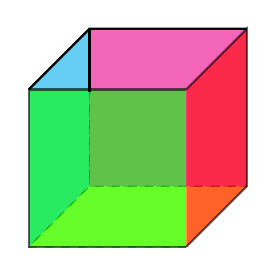
\begin{tikzpicture}
    \coordinate (A0) at (1,1,1);
    \coordinate (A1) at (1,1,-1);
    \coordinate (A2) at (1,-1,1);
    \coordinate (A3) at (1,-1,-1);
    \coordinate (A4) at (-1,1,1);
    \coordinate (A5) at (-1,1,-1);
    \coordinate (A6) at (-1,-1,1);
    \coordinate (A7) at (-1,-1,-1);
    \draw[dashed,fill=cyan,opacity=0.6] (A4) -- (A5) -- (A7) -- (A6);
    \draw[dashed,fill=magenta,opacity=0.6] (A1) -- (A5) -- (A7) -- (A3);
    \draw[dashed,fill=yellow,opacity=0.6] (A2) -- (A6) -- (A7) -- (A3);
    \draw[thick,fill=red,opacity=0.6] (A0) -- (A1) -- (A3) -- (A2);
    \draw[thick,fill=green,opacity=0.6] (A0) -- (A4) -- (A6) -- (A2);
    \draw[thick] (A4) -- (A5) -- (A1);
    \draw[thick] (A5) -- (-1,0.2,-1);
  \end{tikzpicture}
\end{center}

The left figure is a cube, a polyhedron with
six square \textbf{faces}, twelve edges, and eight vertices.
The right is the same, but with the top face removed.
The right figure is not a polyhedron because, like DEF, it leaves ``open ends.''
However, in this case, the open ends are not vertices but the top four edges,
which are each connected to only one face.
We require that within a polyhedron, every edge be connected to exactly two faces.
\footnote{
  Our previous rule for polygons does not apply to the cube or to other polyhedra;
  every vertex of the cube is connected to three edges, not two.
  However, the rule does apply to each of the cube's faces.
}

Are you beginning to see a pattern?
In an $n$-polytope, removing an $(n-1)$-dimensional facet
creates ``open ends'' in the $(n-2)$-dimensional ``facets of facets,'' or \textbf{ridges}.
Ridges are the vertices of polygons, the edges of polyhedra, the faces of polychora, and so on.
Thus the next trait of a polytope is:
\begin{enumerate}
  \setcounter{enumi}{1}
\item Every ridge must be connected to exactly two facets.
\end{enumerate}

Collectively, a polytope's vertices, edges, faces,
and so on are known as its \textbf{elements}.
We may keep track of which elements have which others as facets using a \textbf{Hasse diagram},
shown below for the triangle ABC.

\begin{center}
  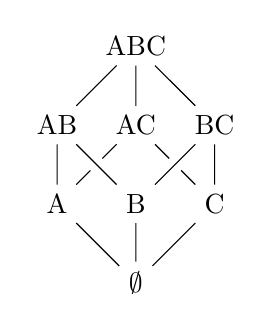
\begin{tikzpicture}
    \node (abc) at (0,3) {ABC};
    \node (ab) at (-1,2) {AB};
    \node (ac) at (0,2) {AC};
    \node (bc) at (1,2) {BC};
    \node (a) at (-1,1) {A};
    \node (b) at (0,1) {B};
    \node (c) at (1,1) {C};
    \node (o) at (0,0) {$\emptyset$};
    \draw (o) -- (a) -- (ab) -- (abc) -- (ac) -- (c)
    (b) -- (o) -- (c) -- (bc) -- (abc)
    (a) -- (ac);
    \draw[preaction={draw=white, -,line width=6pt}] (ab) -- (b) -- (bc);
  \end{tikzpicture}
\end{center}

Each node of the Hasse diagram represents an element of ABC,
including both the whole triangle at the top
and the \textbf{null element} $\emptyset$ at the bottom.
\footnote{
  $\emptyset$, also known as the \textbf{nullitope}, is a convenient edge case.
  It has no vertices or other elements and is considered to be $-1$-dimensional!
}
Whenever two nodes of the diagram are connected,
the higher node's element contains the lower node's element as a facet.
For example, the edge AC contains the vertex C,
so their nodes are connected in the diagram with AC above C.
Notice that the structure of the diagram does not depend on where the vertices are;
a scalene triangle would have the same Hasse diagram as the equilateral ABC.

A diagram considered on its own, without mention of the vertices' locations,
is also known as an \textbf{abstract polytope}.
For example, consider the following diagram:

\begin{center}
  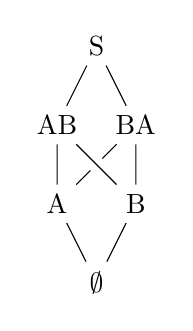
\begin{tikzpicture}
    \node (s) at (0,3) {S};
    \node (ab) at (-0.5,2) {AB};
    \node (ba) at (0.5,2) {BA};
    \node (a) at (-0.5,1) {A};
    \node (b) at (0.5,1) {B};
    \node (o) at (0,0) {$\emptyset$};
    \draw (o) -- (a) -- (ab) -- (s) -- (ba) -- (b) -- (o)
    (a) -- (ba);
    \draw[preaction={draw=white, -,line width=6pt}] (b) -- (ab);
  \end{tikzpicture}
\end{center}

It represents an abstract ``polytope'' with
one null element, two vertices, two edges, and one face (reading from the bottom up).
It satisfies the two conditions given thus far and is often called the digon (two-sided polygon).
However, its two sides AB and BA contain all of the same elements (A, B, and $\emptyset$)
and will lie on top of each other when drawn on a sheet of paper.
For this reason, the digon is not considered a polytope.
Likewise, a quadrilateral with two vertices in the same spot,
which would look like a triangle when drawn, is also not a polytope.
This leads us to the third criterion:

\begin{enumerate}
  \setcounter{enumi}{2}
\item No two elements of the polytope may coincide:
  \begin{enumerate}
  \item no two elements (other than vertices and $\emptyset$) may have the same facets and
  \item no two vertices may have the same location.
  \end{enumerate}
\end{enumerate}

Figures which pass the first and second tests but not this third,
such as the digon, are called \textbf{fissaries}.

Note than condition 3(b) is the first which cannot be tested just from the Hasse diagram.
Condition 1 is equivalent to requiring that the Hasse diagram be organized into ``layers,''
with one element on the top (the whole polytope) and another on the bottom ($\emptyset$)

%% The two criteria of polytopes so far mentioned can be checked
%% just by looking at the corresponding abstract polytope.
%% However, the next part of the definition of a polytope
%% often cannot be checked with just the Hasse diagram.

%% Although every polytope can be represented by a Hasse diagram,
%% not every diagram represents a polytope.
%% For example, removing edge $\overline{\rm BC}$ from $\Delta$ABC
%% produces a new figure (left) and Hasse diagram (right):

%% \begin{center}
%%   \begin{tikzpicture}
%%     \node (a) at (0,0) {A};
%%     \node (b) at (0.5,0.866) {B};
%%     \node (c) at (1,0) {C};
%%     \draw (c) -- (a) -- (b);
%%   \end{tikzpicture}
%%   \begin{tikzpicture}
%%     \node (abc) at (0,2) {ABC};
%%     \node (ab) at (-1,1) {AB};
%%     \node (ac) at (0,1) {AC};
%%     \node (a) at (-1,0) {A};
%%     \node (b) at (0,0) {B};
%%     \node (c) at (1,0) {C};
%%     \node (o) at (0,-1) {$\emptyset$};
%%     \draw (o) -- (a) -- (ab) -- (abc) -- (ac) -- (c)
%%     (b) -- (o) -- (c)
%%     (a) -- (ac);
%%     \draw[preaction={draw=white, -,line width=6pt}] (ab) -- (b);
%%   \end{tikzpicture}
%% \end{center}

%% Note, however, that this requirement applies only to polygons.
%% To generalize it to $n$-polytopes,


\section{Regular polytopes}
There are multiple definitions for when a polytope is \textbf{regular},
but they all require every element (vertices, edges, faces, etc.) to ``look the same.''

\section{Uniform polytopes}
General polytopes can be very complicated. Therefore, we only tend to study specific categories of polytopes. The type of polytopes we study most in this server are \textbf{uniform polytopes}.

Uniformity is defined recursively. In 2D, uniform polytopes are simply the regular polygons.
In higher dimensions, uniform polytopes are the vertex-transitive polytopes whose facets are all uniform. To see what we mean, let's look at a few examples.

\begin{figure}[H]
\centering
\begin{subfigure}{.33333\textwidth}
  \centering
  \includegraphics[width=.5\linewidth]{tut}
  \caption{Truncated tetrahedron\\(tut)}
  \label{fig:tut}
\end{subfigure}%
\begin{subfigure}{.33333\textwidth}
  \centering
  \includegraphics[width=.5\linewidth]{did}
  \caption{Dodecadodecahedron\\(did)}
  \label{fig:did}
\end{subfigure}%
\begin{subfigure}{.33333\textwidth}
  \centering
  \includegraphics[width=.5\linewidth]{snid}
  \caption{Snub icosidodecahedron\\(snid)}
  \label{fig:snid}
\end{subfigure}%
\caption{Three examples of uniform polyhedra. They all have regular polygonal faces (corresponding to the 2D uniforms) and are vertex-transitive.}
\label{fig:uniforms3D}
\end{figure}

In 3D, the uniform polytopes have already been enumerated. It turns out that, aside from the infinite families of \textbf{prisms} and \textbf{antiprisms}, there's exactly 75 uniform polyhedra. % TODO: Link to a listing

\begin{figure}[H]
\centering
\begin{subfigure}{.5\textwidth}
  \centering
  \includegraphics[width=.5\linewidth]{hep}
  \caption{Heptagonal prism (hep)}
  \label{fig:hep}
\end{subfigure}%
\begin{subfigure}{.5\textwidth}
  \centering
  \includegraphics[width=.5\linewidth]{heap}
  \caption{Heptagonal antiprism (heap)}
  \label{fig:heap}
\end{subfigure}%
\caption{An example of a prism and an antiprism. These can be built from any regular polygon, and made uniform in all cases.}
\label{fig:prisms}
\end{figure}

In 4D and higher up, the problem of enumerating the uniforms remains unsolved. As of February 2021, we know of two infinte families plus 2194 uniform polychora. In 5D and up, we haven't yet done a thorough examination, though we know of various constructions that generate uniforms in any dimension.

\subsection{Coxeter Diagrams}


\subsection{Multiprisms}

\section{CRF polytopes}
A polytope is called \textbf{convex regular-faced}, or \textbf{CRF} for short, when it is convex (without dents, holes or self-intersections) and all of its faces are regular. Let's look at a few examples.

\begin{figure}[h]
  \centering
  \begin{subfigure}{.33333\textwidth}
    \centering
    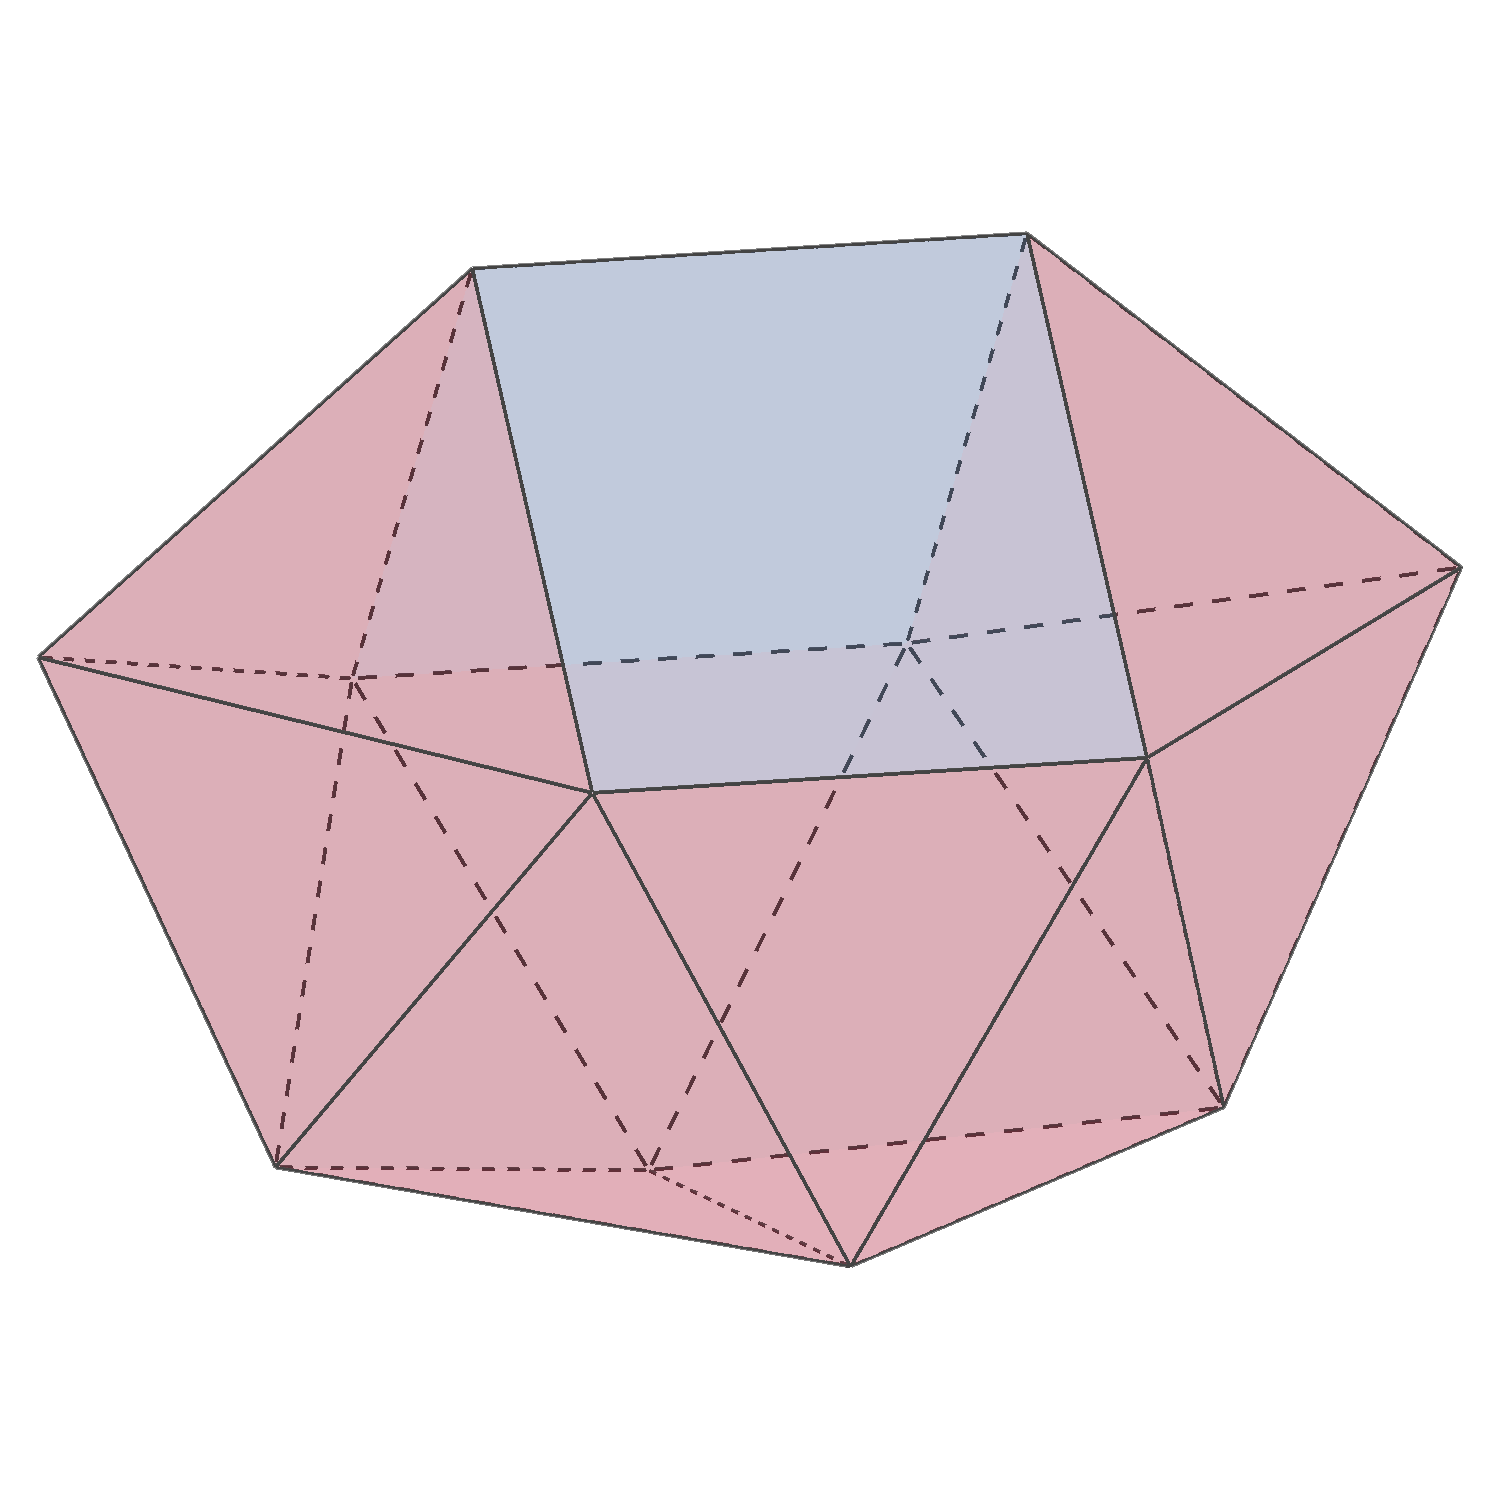
\includegraphics[width=.5\linewidth]{Sphenomegacorona}
    \caption{Sphenomegacorona}
    \label{fig:polyhedra_1}
  \end{subfigure}%
  \begin{subfigure}{.33333\textwidth}
    \centering
    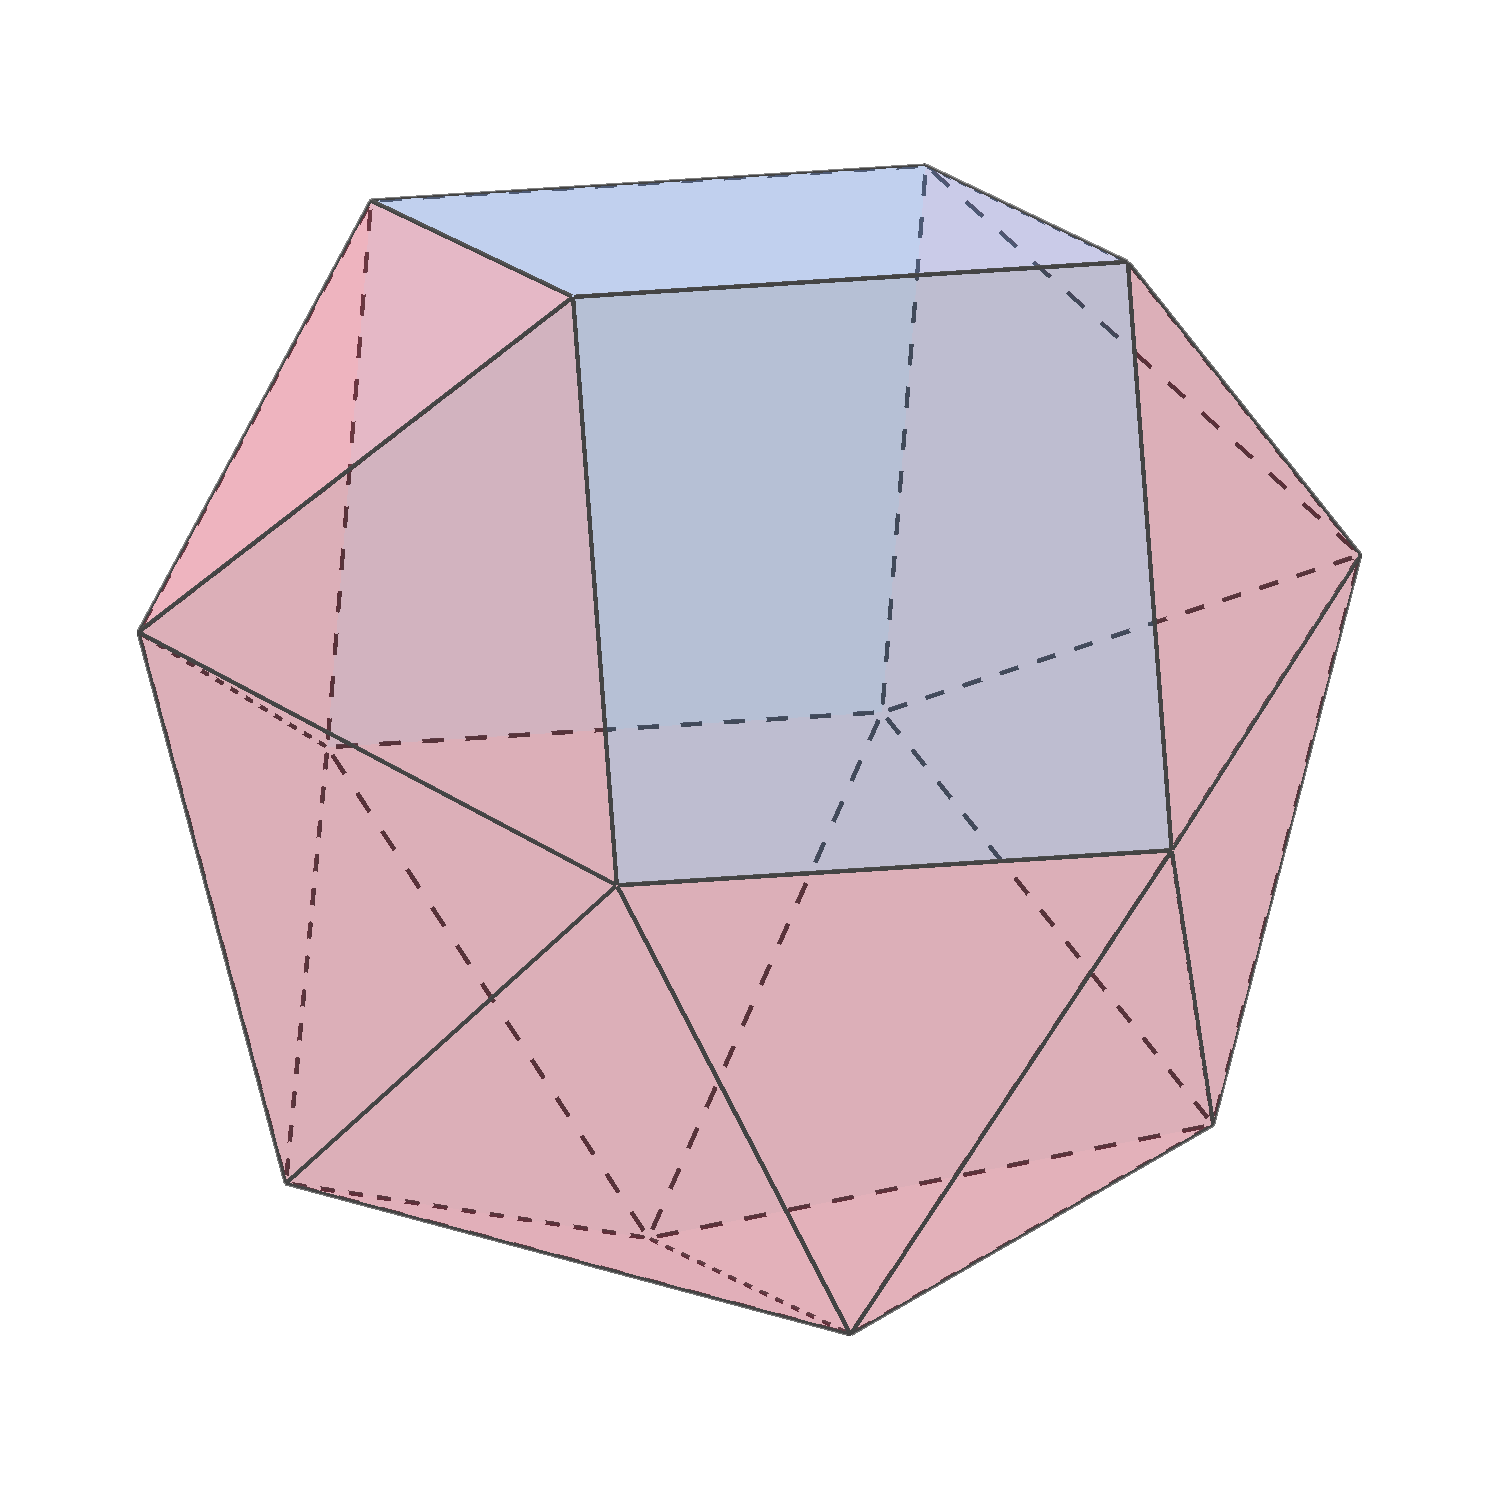
\includegraphics[width=.5\linewidth]{Hebesphenomegacorona}
    \caption{Hebesphenomegacorona}
    \label{fig:polyhedra_2}
  \end{subfigure}%
  \begin{subfigure}{.33333\textwidth}
    \centering
    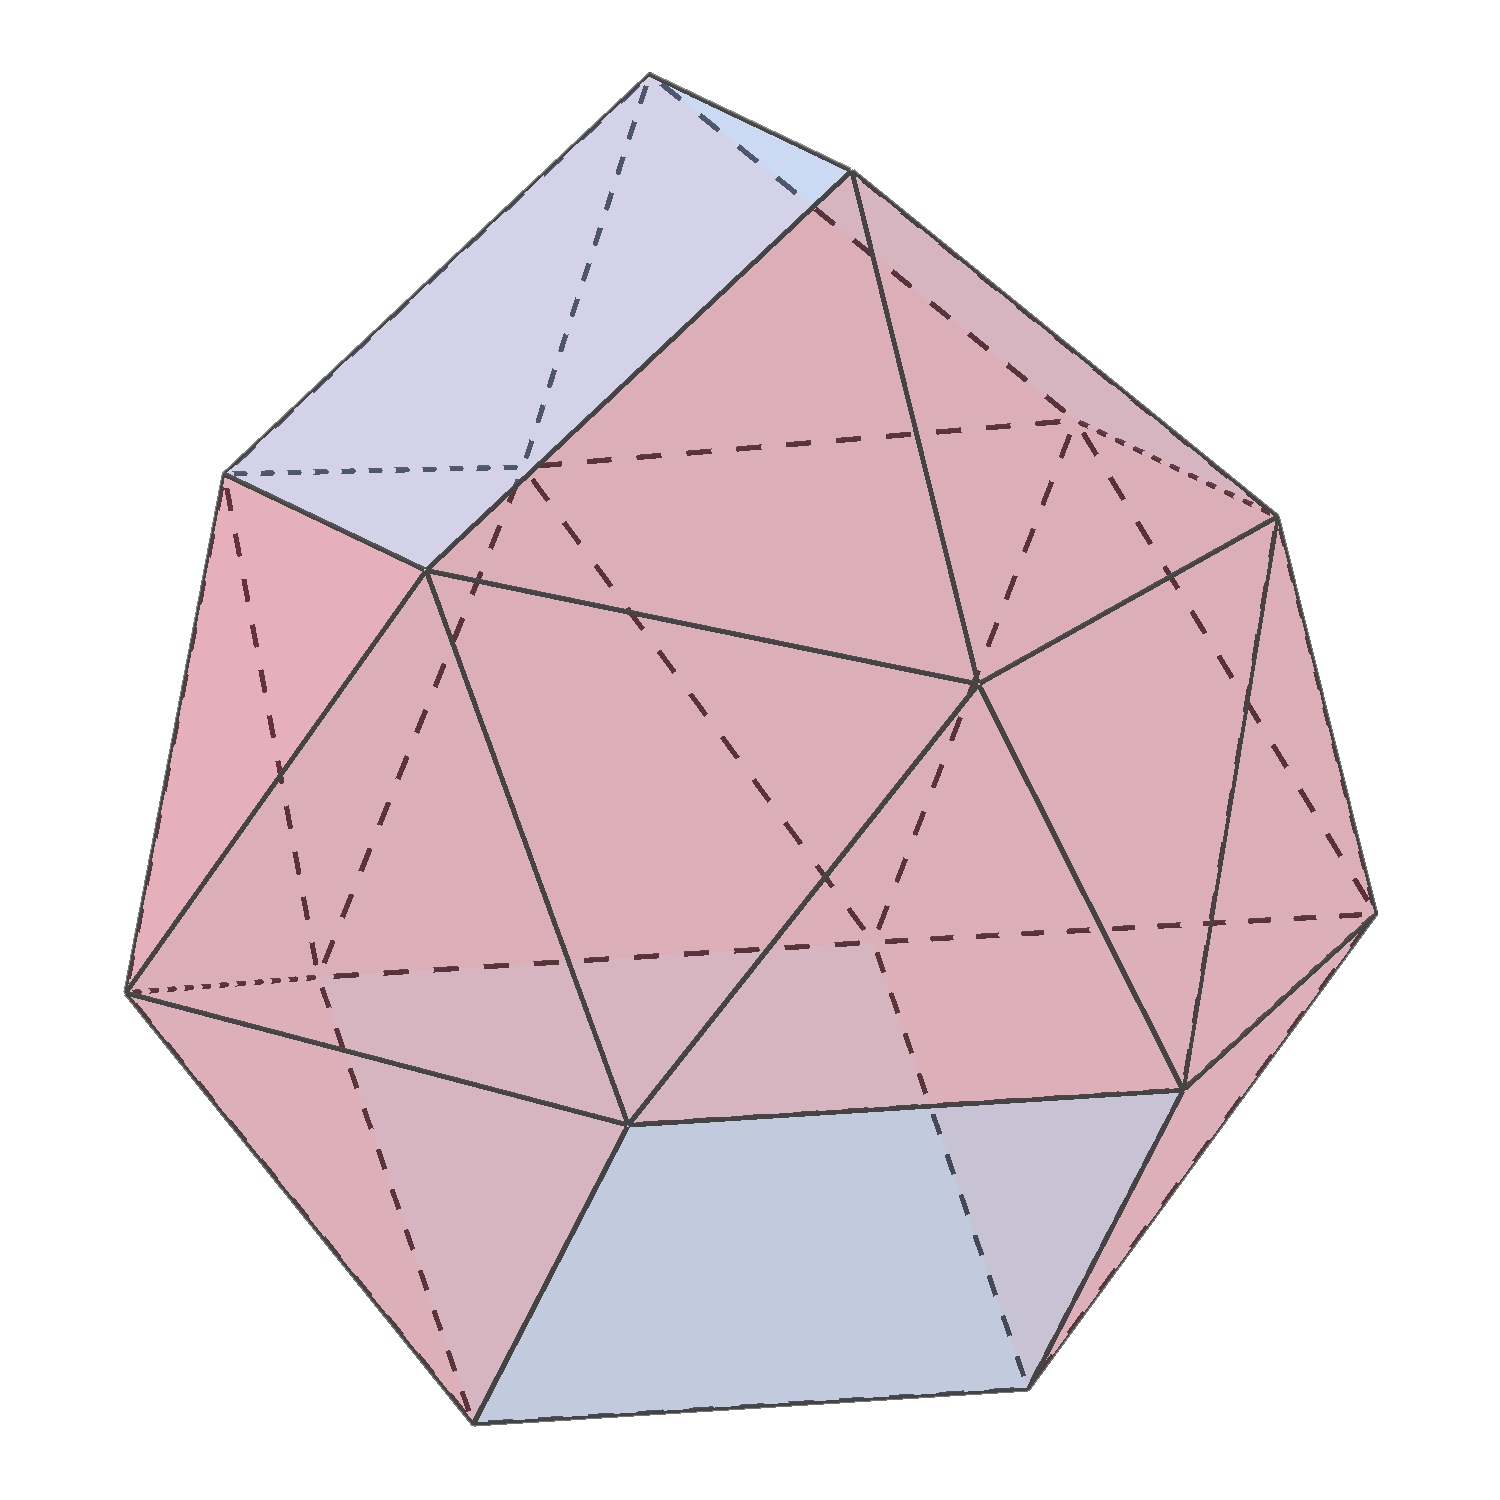
\includegraphics[width=.5\linewidth]{Disphenocingulum}
    \caption{Disphenocingulum}
    \label{fig:polyhedra_3}
  \end{subfigure}%
  \caption{Test images!}
  \label{fig:polyhedra}
\end{figure}

\end{document}
